%!TEX TS-program = xelatex
\documentclass[aspectratio=169,newPxFont]{beamer}
%\documentclass[newPxFont,handout]{beamer} % Раздаточный материал (на слайдах всё сразу)
%\documentclass[aspectratio=169]{beamer} % Соотношение сторон

\usetheme{LTX}

%-=-=-=-=-=-=-=-=-=-=-=-=-=-=-=-=-=-=-=-=-=-=-=-=
%        LOADING PACKAGES
%-=-=-=-=-=-=-=-=-=-=-=-=-=-=-=-=-=-=-=-=-=-=-=-=
\usepackage{amsmath,amsfonts,amssymb,amsthm,mathtools}  % Тут мы подключаем пакеты для математики!
\usepackage{wasysym}
%%%%%%%%%%%%%%%%%%%%%%%% Шрифты %%%%%%%%%%%%%%%%%%%%%%%%%%%%%%%%%

\usepackage{fontspec}         % пакет для подгрузки шрифтов
\setmainfont{Helvetica}  % задаёт основной шрифт документа

% why do we need \newfontfamily:
% http://tex.stackexchange.com/questions/91507/
\newfontfamily{\cyrillicfonttt}{Helvetica}
\newfontfamily{\cyrillicfont}{Helvetica}
\newfontfamily{\cyrillicfontsf}{Helvetica}
% Иногда тех не видит структуры шрифтов. Эти трое бравых парней спасают ситуацию и доопределяют те куски, которые Тех не увидел.

% \usepackage{unicode-math}     % пакет для установки математического шрифта
% \setmathfont{Asana Math}      % шрифт для математики

\usepackage{polyglossia}      % Пакет, который позволяет подгружать русские буквы
\setdefaultlanguage{russian}  % Основной язык документа
\setotherlanguage{english}    % Второстепенный язык документа

%%% Работа с картинками
\usepackage{graphicx}  % Для вставки рисунков
\graphicspath{{images/}{images2/}}  % папки с картинками
\setlength\fboxsep{3pt} % Отступ рамки \fbox{} от рисунка
\setlength\fboxrule{1pt} % Толщина линий рамки \fbox{}
\usepackage{wrapfig} % Обтекание рисунков текстом

%%% Работа с таблицами
\usepackage{array,tabularx,tabulary,booktabs} % Дополнительная работа с таблицами
\usepackage{longtable}  % Длинные таблицы
\usepackage{multirow} % Слияние строк в таблице

%%% Программирование
\usepackage{etoolbox} % логические операторы

%%% Другие пакеты
\usepackage{multicol} % Несколько колонок

%%% Картинки
\usepackage{tikz} % Работа с графикой
\usepackage{pgfplots}
\usepackage{pgfplotstable}


\usepackage{xcolor}
\usepackage{hyperref}
\hypersetup{
    unicode=true,           % позволяет использовать юникодные символы
    colorlinks=true,       	% true - цветные ссылки, false - ссылки в рамках
    urlcolor=blue,          % цвет ссылки на url
    linkcolor=red,          % внутренние ссылки
	hyperindex=true,        % сделать ли ссылку кликабельной?
	breaklinks=true         % если ссылка не умещается в одну строку, разбивать
	                        % ли ее на две части?
}
\usepackage{verbatim}
\usepackage{fancyvrb}
\usepackage{mdframed}


\usepackage{chronology}

\renewcommand{\event}[3][e]{%
  \pgfmathsetlength\xstop{(#2-\theyearstart)*\unit}%
  \ifx #1e%
    \draw[fill=black,draw=none,opacity=0.5]%
      (\xstop, 0) circle (.2\unit)%
      node[opacity=1,rotate=45,right=.2\unit] {#3};%
  \else%
    \pgfmathsetlength\xstart{(#1-\theyearstart)*\unit}%
    \draw[fill=black,draw=none,opacity=0.5,rounded corners=.1\unit]%
      (\xstart,-.1\unit) rectangle%
      node[opacity=1,rotate=45,right=.2\unit] {#3} (\xstop,.1\unit);%
  \fi}%


\title{Уютный факультатив по \LaTeX}
\subtitle{Введение в \LaTeX}
\date{\today}

\begin{document}

\begingroup
\setbeamercolor{background canvas}{bg = LTXDarkGrey}
\begin{frame}[plain]
\begin{center}
\Huge{\color{red}{ВНИМАНИЕ!}}
\end{center}

\begin{center}
\color{white}{ДАННЫЙ КУРС СОДЕРЖИТ БОЛЬШОЕ КОЛИЧЕСТВО РАЗНООБРАЗНОГО КОДА И ЗАДАНИЙ ДЛЯ САМОСТОЯТЕЛЬНОГО РЕШЕНИЯ. \\
\vspace{3mm}
НА ПЕРВЫЙ ВЗГЛЯД ОН МОЖЕТ ПОКАЗАТЬСЯ СЛОЖНЫМ И ТРАВМИРОВАТЬ НЕПОДГОТОВЛЕННУЮ ПСИХИКУ. ТАКЖЕ ОН СОДЕРЖИТ БОЛЬШОЕ КОЛИЧЕСТВО НЕУДАЧНЫХ ШУТОК И НЕУМЕСТНЫХ ОТСЫЛОК. \\ 
\vspace{3mm}
В СВЯЗИ С ЭТИМ КУРС НЕ РЕКОМЕНДУЕТСЯ ПРОСЛУШИВАТЬ \ldots{ } НИКОМУ.}
\end{center}
\end{frame}
\endgroup

 \maketitle

\begin{frame}
\frametitle{Идеология курса}
\begin{itemize}
\item 8 лекций и 7 семинаров
\item что-то неясно $\Rightarrow$ \alert{ ПЕРЕБЕЙ И СПРОСИ}
\item на семинаре присутствуют 3-5 человек, которые хорошо знают \LaTeX{} и помогают вам
\item есть проблема $\Rightarrow$ \alert{ЗОВИ ОДНОГО ИЗ НАС} 
\item пять обязательных заданий и два необязательных 
\item все по 20 баллов, для зачёта надо 70\% 
\end{itemize}
\end{frame}


\begin{frame}
\frametitle{План, по которому всё пойдёт}
\begin{enumerate}
\item Обо всём и ни о чём! Мотивация, математика, шрифты
\item Картинки, таблицы, графика, TikZ, Geogebra
\item Оформление документа в целом
\item Список литературы.  Преамбула для души и по ГОСТ
\item Немного своих команд и макросов. 
\item Связка R и \LaTeX{}. Красивая эконометрика
\item Связка R и \LaTeX{}. Автоматизация создания документов
\item Презентации. Atom, Markdown и Rshiny,  всякие мелочи.
\end{enumerate}
\end{frame}


\begin{frame}
\frametitle{Куда идти за мудростью}

У нашего курса есть страничка на Github! Многие из вас уже были там и видели, что там много разной мудрости.
\vspace{1cm}

\begin{block}{Страничка курса:}
\vspace{3mm}
\centerline {\url{https://fulyankin.github.io/LaTeX/}}
\vspace{3mm}
\end{block}
\end{frame}


\begin{frame}
\frametitle{Что это вообще такое ?}
\alert{TeX} —  это созданная американским математиком и программистом Дональдом Кнутом система для верстки текстов с формулами.

\centering 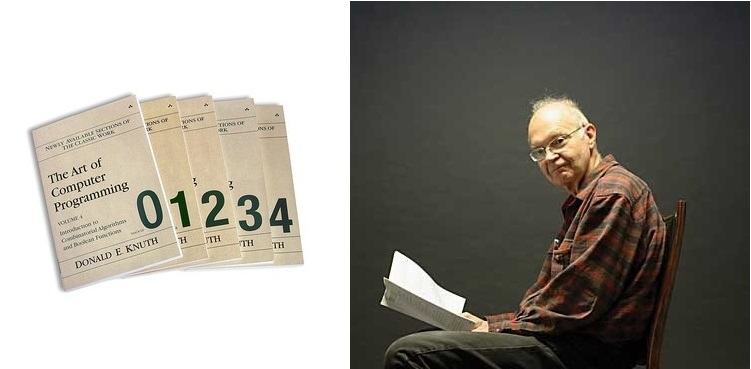
\includegraphics[scale=0.5]{knut.jpg}\\
\end{frame}


\begin{frame}
\frametitle{Почему \LaTeX{}?}
\begin{itemize}
\item Он позволяет делать красивые документы
\item Особенно документы с формулами
\item Он был создан учёными для учёных
\item Большое и активное комьюнити, у которого всегда можно попросить о помощи
\item Он уютный!
\item Многие вещи, связанные с оформлением автоматизированы, что позволяет думать о содержании
\item Огромное количество различных пакетов и расширений в свободном доступе
\end{itemize}
\end{frame}


\begin{frame}
\frametitle{Откуда появился \LaTeX{}?}
\begin{columns}
\begin{column}{.48\linewidth}
\centering 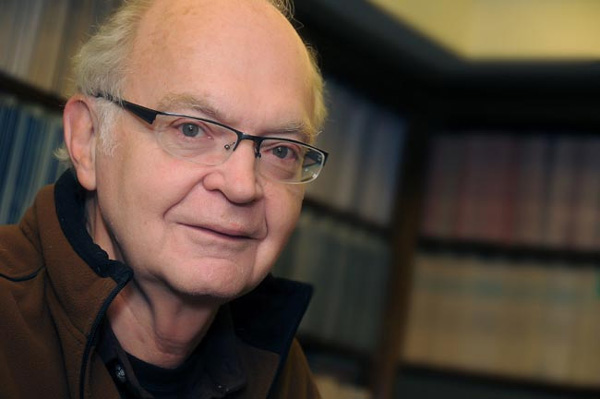
\includegraphics[scale=0.2]{DK.jpg}\\
\mbox{ } \\
Дональд Кнут создал в 1978 году программу \TeX.
\end{column}

\begin{column}{.48\linewidth}
\centering Лесли Лэмпорт создал в 1984 году макропакет \LaTeX. \\
\mbox{ } \\
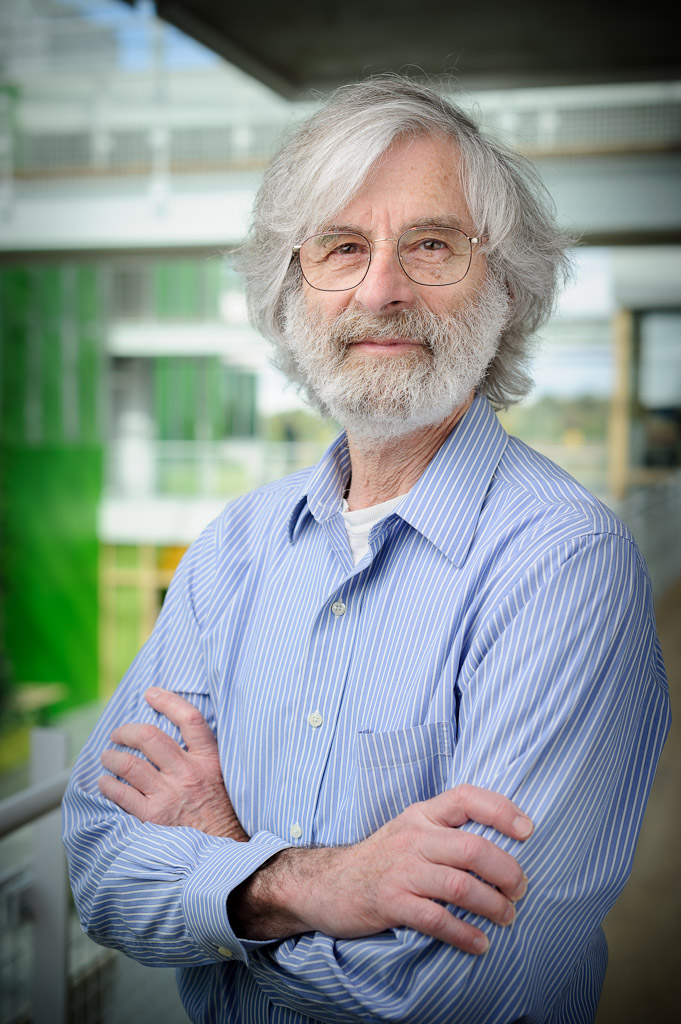
\includegraphics[scale=0.4]{LL.jpg}
\end{column}
\end{columns}
\end{frame}


\begin{frame}{Движки}
\centering
	\begin{tabulary}{\textwidth}{JcJ}
		\toprule
			движок			& рождение & отличия	\\[0.25em]
		\midrule
		\TeX{}				    & 1978 & начало пути  \\[0.25em]
		\LaTeX{}				& 1984 & расширение, упрощение \\[0.25em]
		\midrule

		pdf\LaTeX{}				& 2000 & сборка не dvi, а сразу pdf  \\[0.25em]
		Xe\LaTeX{}				& 2004 & юникод, куча шрифтов   \\[0.25em]
		Lua\LaTeX{} 		    & 2007 & язык Lua + Xe\LaTeX     \\[0.25em]
		\midrule
		bib\TeX{}				& 1985 &  удобная библиография  \\[0.25em]
		bib\LaTeX{} (biber)		& 2010 &  юникод, ряд улучшений    \\[0.25em]
		\bottomrule
	\end{tabulary}

	\href{https://habrahabr.ru/post/114610/}{Статья про движки на хабре}
\end{frame}


\begin{frame}{О правильном софте}
\begin{columns}
\begin{column}{.48\linewidth}
\centering

\includegraphics[width=0.4\linewidth]{RStudio-Ball.png}\\
\mbox{ } \\

\includegraphics[width=0.9\linewidth]{Python-logo.png}\\
\end{column}


\begin{column}{.48\linewidth}
\centering

\includegraphics[width=0.5\linewidth]{julia-logo.png}
\mbox{ } \\

\includegraphics[width=0.7\linewidth]{c-vs-cpp.png}
\end{column}
\end{columns}
\end{frame}


\begin{frame}{Популярность языков программирования}
\centering 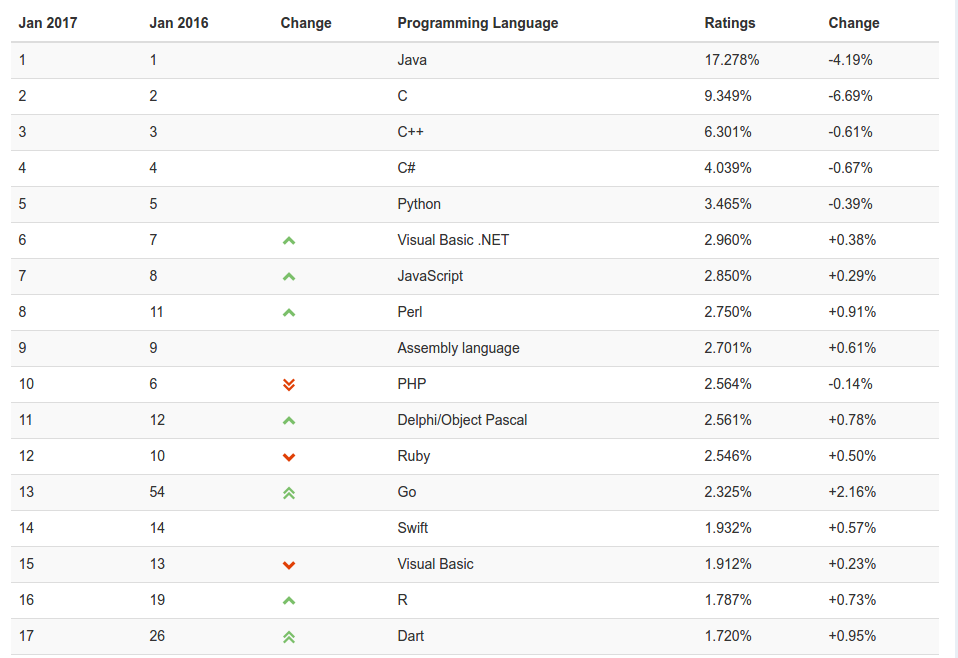
\includegraphics[width=0.6\linewidth]{lang.png}\\
\vspace{0.2cm}
Подробнее на {\url{http://www.tiobe.com/tiobe-index/}}
\end{frame}


\begin{frame}{Самый важный язык}
\centering 
\includegraphics[width=0.7\linewidth]{english.jpg}\\
\end{frame}


\begin{frame}{How to \ldots а также Error: \ldots}
\centering 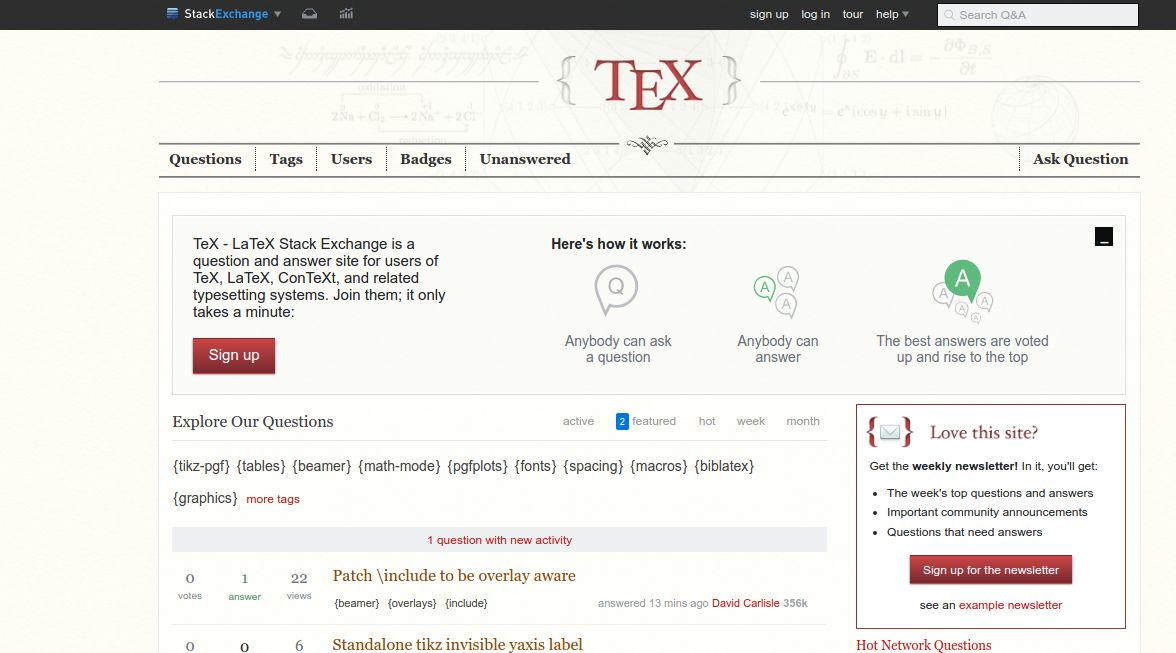
\includegraphics[width=0.8\linewidth]{texexchan.png}\\
\end{frame}


\begin{frame}{Мой рук}
\centering 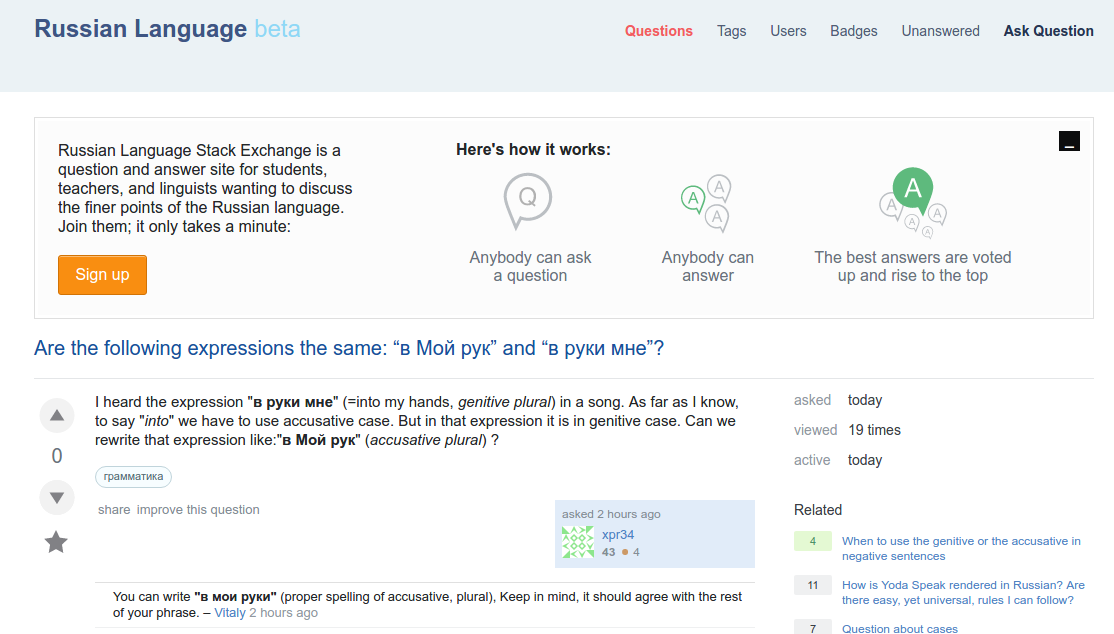
\includegraphics[width=0.8\linewidth]{russia.png}\\
\end{frame}


% \begin{frame}{Мемы про Stack Overflow}
% \begin{columns}
% \begin{column}{.48\linewidth}
% 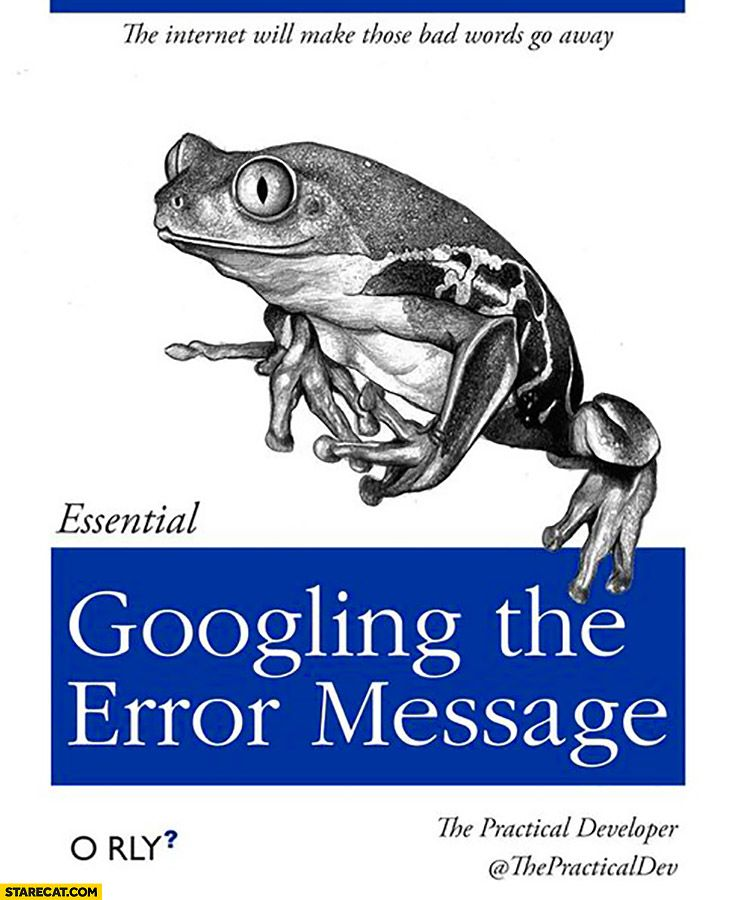
\includegraphics[width=0.8\linewidth]{googling.jpg}\\
% \end{column}
% \begin{column}{.48\linewidth}
% includegraphics[width=0.8\linewidth]{copypast.jpg}\\
% \end{column}
% \end{columns}
% \end{frame}


\begin{frame}
\frametitle{Особенности \LaTeX}
\LaTeX{} не WYSIWYG (What You See Is What You GET)
В WYSIWYG системах что автор видит на экране, то и получается на печати.

\mbox{ }

\LaTeX{} WYSIWYM (What You See Is What You \alert{MEAN})
\LaTeX{} сам позаботится об оформлении, вам остаётся только думать о содержании!
\end{frame}



\begin{frame}[fragile]
\frametitle{Как это работает?}
Вы пишите свой текст с различными \alert{командами}, описывающими структуру текста, а \LaTeX{} преобразует их в красиво отформатированный pdf-документ!

\begin{mdframed}[backgroundcolor=LTXLightGreen]
В Португалии \verb|\textbf|\{дождь\} является \verb|\textit|\{причиной\}  не выходить на работу.
\end{mdframed}

\centering
   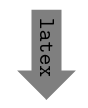
\includegraphics[scale=0.3]{fuc.png}%}

\begin{mdframed}[backgroundcolor=LTXLightGreen]
В Португалии \textbf{дождь} является \textit{причиной} не выходить на работу.
\end{mdframed}
\end{frame}

\begin{frame}[fragile]
\frametitle{Ещё примеры работы \LaTeX{}!}

\begin{tabular}{p{7cm}p{4cm}}
\vspace{10mm} \verb|
\includegraphics[scale=0.15]{doge.png}| &  \begin{center} 
\includegraphics[scale=0.2]{doge.png} \end{center}
\end{tabular}
\vspace{3mm}
\begin{tabular}{p{7cm}p{4cm}}
\centering \verb|$\alpha^{x+5} + \sigma_{t}$| & \centering  $\alpha^{x+5}+\sigma_{t}$
\end{tabular}
\end{frame}



\begin{frame}[fragile]
\frametitle{Любой документ состоит из двух частей!}
\begin{mdframed}[backgroundcolor=LTXLightGreen]
\verb|\documentclass[12pt, a4paper]{article}|\\
\\
\% Тут располагается преамбула документа!\\
\\
\verb|\begin{document}|\\
\\
\% Тут располагается сам документ!\\
\\
\verb|\end{document}|\\
\end{mdframed}
\end{frame}


\begin{frame}{Что где писать}
\begin{block}{Преамбула}
\begin{itemize}
\item Команды, определяющие вид документа в целом
\item Команды, подключающие пакеты
\item Команды, которые создают новые команды, чтобы удобнее использовать старые команды
\item Ещё какие-нибудь команды
\end{itemize}
\end{block}

\begin{block}{Документ}
Основной текст документа
\end{block}
\end{frame}


\begin{frame}{Откуда берутся пакеты?}

\begin{columns}
\begin{column}{.66\linewidth}
\begin{itemize}
\item Их находят в капусте (нет)
\item Их скачивают с сайта \url{http://www.ctan.org}
\end{itemize}
\end{column}
\begin{column}{.33\linewidth}
\hfill 
\includegraphics[width=0.6\linewidth]{cabage.png}
\end{column}
\end{columns}
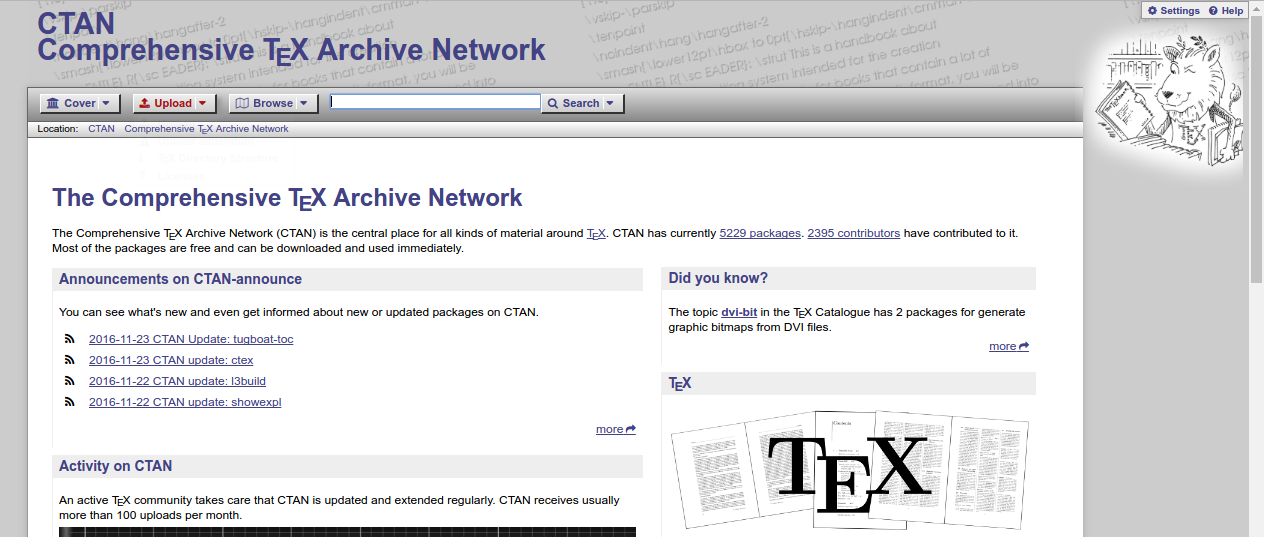
\includegraphics[width=0.6\linewidth]{CTAN.png}
\end{frame}


\begin{frame}[fragile]
\frametitle{Хорошие мысли о \LaTeX!}
\begin{itemize}
\item Каждый документ состоит из преамбулы и основной части; \pause
\item \textbf{Не надо каждый раз писать преамбулу с нуля!}
\item Все \alert{комнады} начинаются с знака \verb|\|; \pause
\item Аргументы команд стоят в фигурных скобках \{ \}; \pause
\item С помощью знака \% можно закомментировать какую-то часть документа, \LaTeX{} проигнорирует закомментированную часть; \pause
\item Неважно сколько строк я оставил между абзацами и сколько пробелов я оставил между словами;
\end{itemize}
\end{frame}

\section{Наш первый файл}
% Cоздаём первый файл до интеграла

\begin{frame}{Компиляция и её результаты}

\centering
	\begin{tabulary}{\linewidth}{JcJ}
		\toprule
		  файл	  & & предназначение \\[0.25em]
		\midrule
		  .tex    & & мы пишем в этом файле  \\[0.25em]
		  .pdf    & & наш документ  \\[0.25em]
		  .log    & & логи, информация обо всём, что произошло во время компиляции  \\[0.25em]
		  .aux    & & карта документа, в нём записаны все ссылки, номера страниц, табоиц и т.д.  \\[0.25em]
          .synctex     & & позволяет нажать в pdf правую кнопку и перейти к соответствующему месту в tex-файле  \\[0.25em]
		\bottomrule
	\end{tabulary}
\end{frame}

\begin{frame}[fragile]
\frametitle{Формулы в \LaTeX!}
\begin{itemize}
\item С помощью символа \$ мы можем перейти внутри текста в математический режим! Один \$ открывает математический режим, второй закрывает его!  \pause
\item С помощью символов \$\$ или \verb|\[| и \verb|\]| можно написать выключную формулу. Выключной объект --- такой объект, для которого необходима отдельная строка! \pause
\item Внутри математического режима \LaTeX{} сам расставляет пробелы. Все ваши пробелы игнорируются.
\end{itemize}
\end{frame}

% Смотрим кусок с интегралом!

\begin{frame}
\frametitle{Формулы в \LaTeX!}
\begin{itemize}
\item В \LaTeX{} можно найти символы на все случаи жизни $\Im$
\item По {\color{blue} \href{http://detexify.kirelabs.org/classify.html}{этой ссылке}} расположен распознаватель символов! \pause
\item В книге Львовского есть огровное количество символов с подробными комментариями! Например:
\end{itemize}

\centering  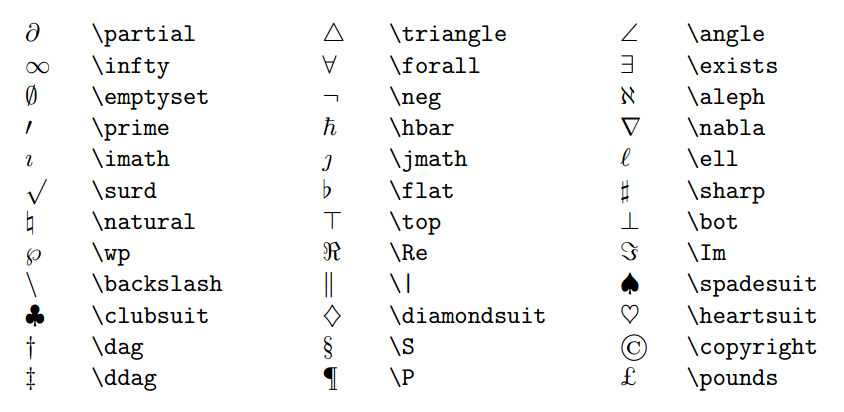
\includegraphics[scale=0.2]{table.png}
\end{frame}

% Распознать символ и вставить его

\begin{frame}
\frametitle{Служебные символы}

\mbox{ }

\centering
\Large{ \$ \% \{ \} \# \& — служебные символы}

\mbox{ }

\begin{itemize}
\item \normalsize{Чтобы использовать \$ или другой символ в тексте, надо написать $\setminus$\$.}
\end{itemize}
\end{frame}


\section{Мотивация}

\begin{frame}{Мотивация}
    \centering
    
\includegraphics[scale=0.5]{m7.png}

	\mbox{ }

    
\includegraphics[scale=0.6]{m9.png}

    \vfill
    \alert{\textbf{В \LaTeX{} никогда ничего никуда не съедет!}}
\end{frame}


\begin{frame}{Мотивация}
    \centering
    
\includegraphics[scale=0.6]{m8.png}

    \vfill
    \alert{\textbf{В \LaTeX{} ничего не изменится и не исчезнет без вашего ведома!}}
\end{frame}


\begin{frame}{Мотивация}
    \centering
    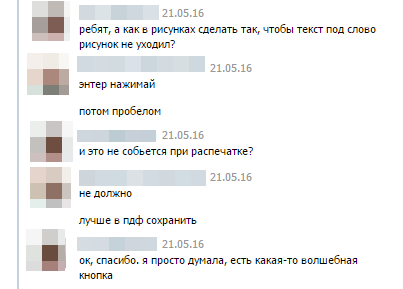
\includegraphics[height=0.6\textheight]{m6.png}

    \vfill
    \alert{\textbf{В \LaTeX{} вы навсегда забудете о "сначала энтер, потом 4 раза пробел"!}}
\end{frame}


\begin{frame}{Мотивация}
    \centering
    \alert{\textbf{В \LaTeX{} список литературы сгенерируется автоматически!}}

    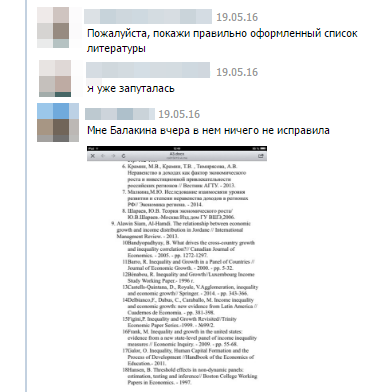
\includegraphics[height=0.68\textheight]{m2.png}
\end{frame}

\begin{frame}{Мотивация}
    \centering
    \alert{\textbf{Зачем первак, когда есть \LaTeX{}!}}

    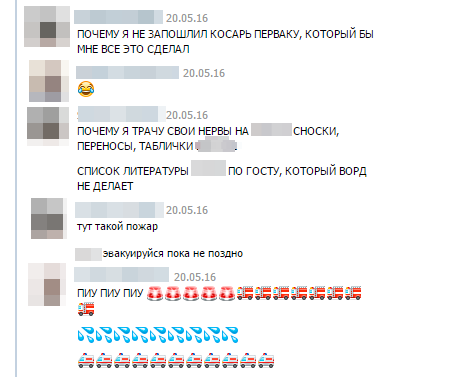
\includegraphics[height=0.68\textheight]{m4.png}
\end{frame}


\begin{frame}{Мотивация}
    \centering
    
\includegraphics[scale=0.8]{m5.png}

    \vfill
    \alert{\textbf{В \LaTeX{} можно написать абсолютно любой шаблон!}}
\end{frame}


\begin{frame}{Где раздобыть шаблоны}
\centering
\url{http://www.latextemplates.com/}


\includegraphics[width=0.4\linewidth]{template1.png}

\url{https://www.overleaf.com/latex/templates}

\includegraphics[width=\linewidth]{template2.png}
\end{frame}


\begin{frame}{Мотивация}
    \centering
    
\includegraphics[scale=0.5]{m10.png}

    \vfill
    \alert{\textbf{А ещё то ли \LaTeX{} то ли ГОСТ придумали рептилоиды!}}
\end{frame}


\begin{frame}{А если говорить серьёзно, то \ldots}
    \centering
    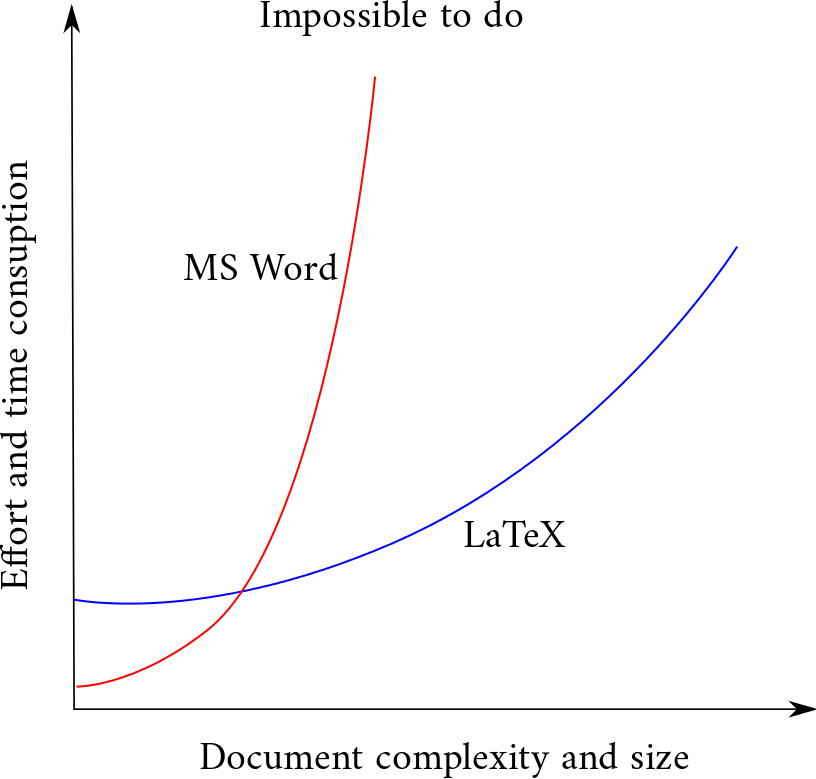
\includegraphics[scale=0.2]{latexvsword.png}
\end{frame}



\begin{frame}{Точка пересечения слишком близко}
\centering
    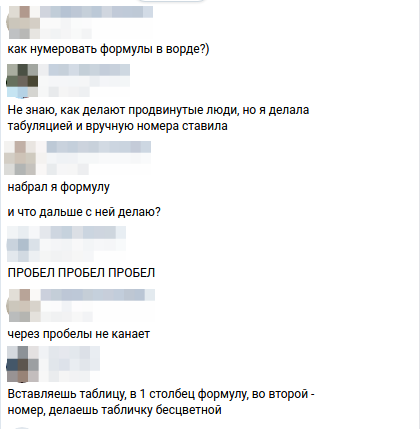
\includegraphics[scale=0.45]{pain.png}


\url{http://www.kgasuclan.ru/blog/119-avtonumeracija-formul-risunkov-tablic-v-word.html}
\end{frame}


\begin{frame}{Если надо совсем простое}
\centering
    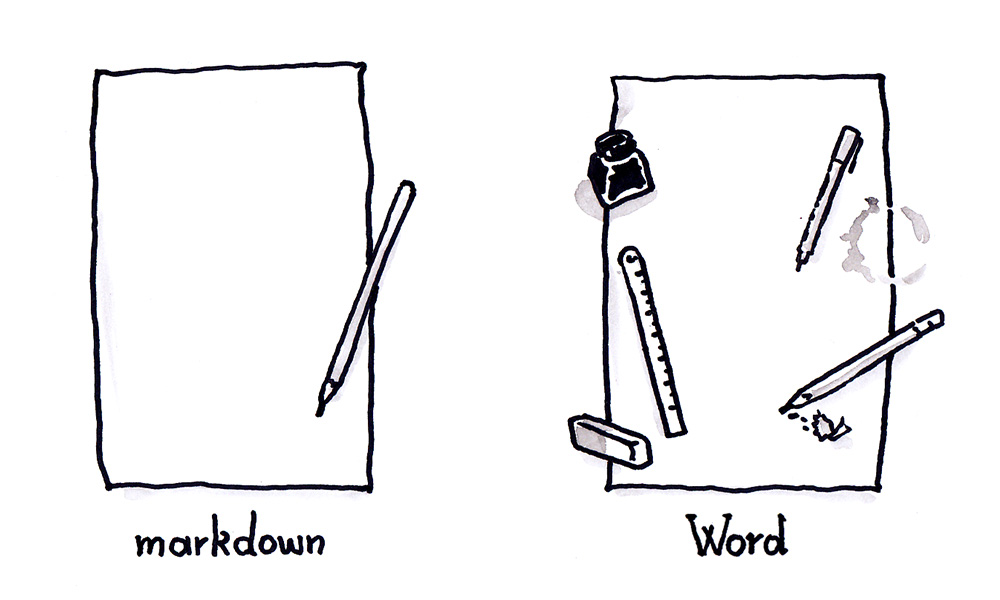
\includegraphics[scale=0.3]{markdown_vs_word.jpg}
\end{frame}


\section{Шрифты}  

\begingroup
\setbeamercolor{background canvas}{bg = LTXDarkGrey}
\begin{frame}[plain]
\centering  
\includegraphics[width=0.63\linewidth]{font.jpg}	
\end{frame}
\endgroup 

\begin{frame}{Кодировка} 
Кодировка - способ представления в памяти компьютера цифр, букв и всех остальных знаков. 

\centering 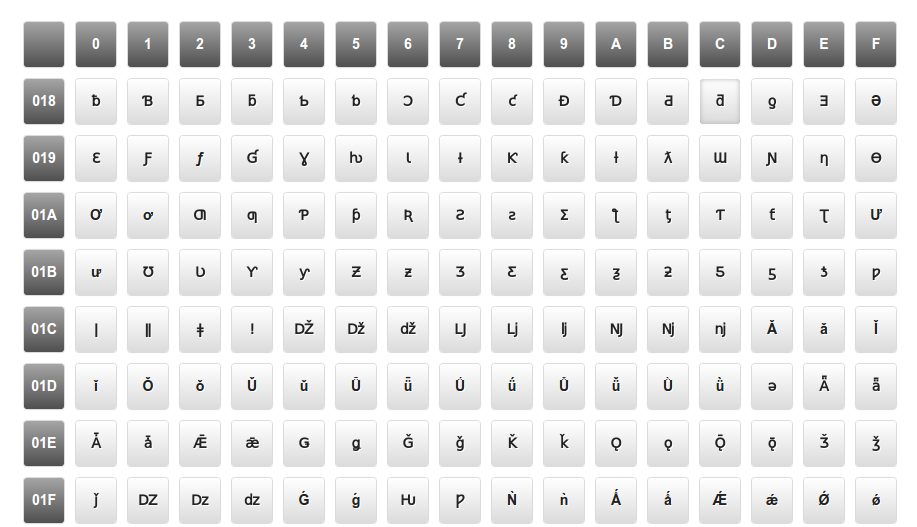
\includegraphics[width=0.68\linewidth]{codirovka.png}	
\end{frame}

\begin{frame}{Откуда берутся кракозябры} 
\centering 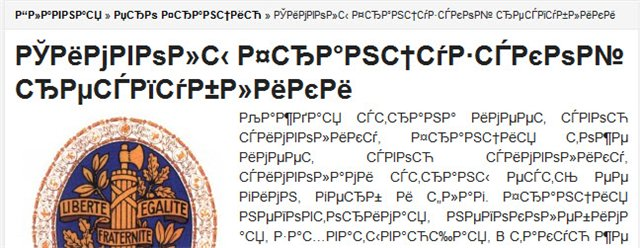
\includegraphics[width=0.7\linewidth]{krakozabr.jpg}	
\vspace{0.3cm}

\begin{itemize}
\item Мало памяти, 7 бит достаточно для всего (256 ячеек)
\item 127 ячеек - основа: символы, цифры, латиница
\item 128 ячеек - другое: кириллица, немецкий и т.п.
\item Каждое новое заполнение 128 символов $\Rightarrow$ новая кодировка
\end{itemize}
\end{frame}


\begin{frame}{Юникод} 
\begin{itemize}
\item Собрались великие умы в 1991 году и юникод придумали!
\end{itemize}

\centering  
\includegraphics[width=0.7\linewidth]{stdcom.jpg}	
\end{frame}


\begin{frame}{Мольба к аудитории}
\begin{columns}
\begin{column}{.66\linewidth}
\Large Весь мир уже давно перешёл на utf-8! Будьте прогрессивными! Плиз... 
\end{column}
\begin{column}{.33\linewidth}
\hfill 
\includegraphics[width=\linewidth]{cuputf8.jpg}	
\end{column}
\end{columns}
\end{frame}


\begin{frame}[fragile]{Старый путь}
\large Самые первые строки в другом движке будут: 
\begin{block}{Движок pdf-LaTeX}
\begin{verbatim}
\usepackage[british,russian]{babel}  % выбор языка
\usepackage[utf8]{inputenc}          % utf8 кодировка
\usepackage[X2,T2A]{fontenc}         % ещё кодировка
\end{verbatim}
\end{block}
\end{frame}

% Показываю файл со шрифтами и их подключением, виньетки для fontspect и для math-unicode
% Показать ссылки на документацию пакетов
% https://www.ctan.org/pkg/fontspec
% https://www.ctan.org/pkg/unicode-math

{
\usebackgroundtemplate{%
\tikz\node[opacity=0.15] {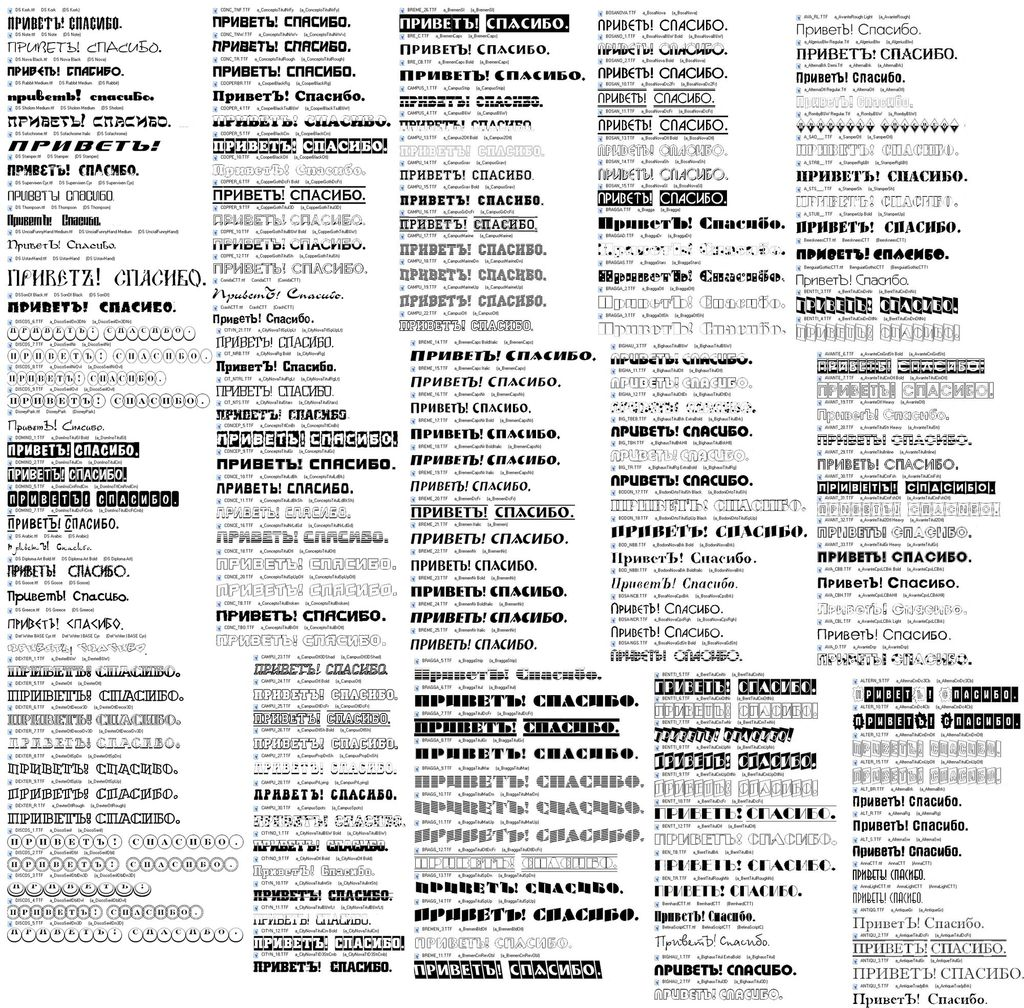
\includegraphics[width=\paperwidth]{bakcfont.jpg}};}
\begin{frame}{Откуда берутся шрифты}
\Large
\begin{itemize}
\item Шрифты скачиваются из интернета \ldots
\item Хорошая идея - установить на комп шрифтовый менеджер для безболезненного просмотра шрифтов
\item Хороший \href{https://apps.ubuntu.com/cat/applications/precise/font-manager/}{ шрифтовый менеджер} для Linux 
\item Хороший \href{http://fontba.se/}{ шрифтовый менеджер} для Windows 
\end{itemize}
\end{frame}
}


\section{Подробнее о математике в \LaTeX{}}


\section{Домашка} 


\begingroup
\setbeamercolor{background canvas}{bg = LTXDarkGrey}
\begin{frame}[plain]
\vspace{0.5cm}
\centering \color{white}{\Huge{ KEEP CALM }}

\vspace{0.2cm}
\centering 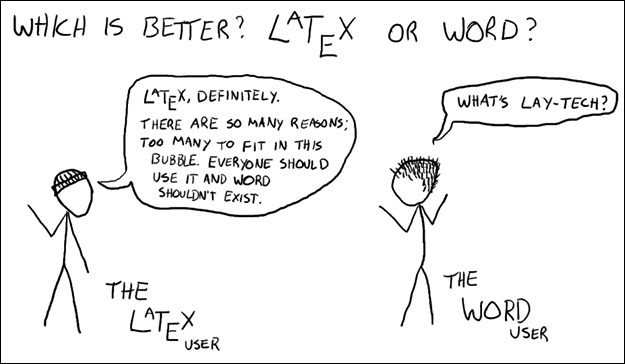
\includegraphics[width=0.7\linewidth]{joke_2.png}
\vspace{0.2cm}

\centering \color{white}{\Huge{ AND \TeX{ } IT }}
\end{frame}
\endgroup

\end{document}
